\begin{pastexam}[label={px:ncku-114-prog-08}]{成大資訊聯招 114 學年度 第 8 題}
（複選；至少有二個正確答案）

{[4\%]} Consider the following AVL tree.

\begin{center}%
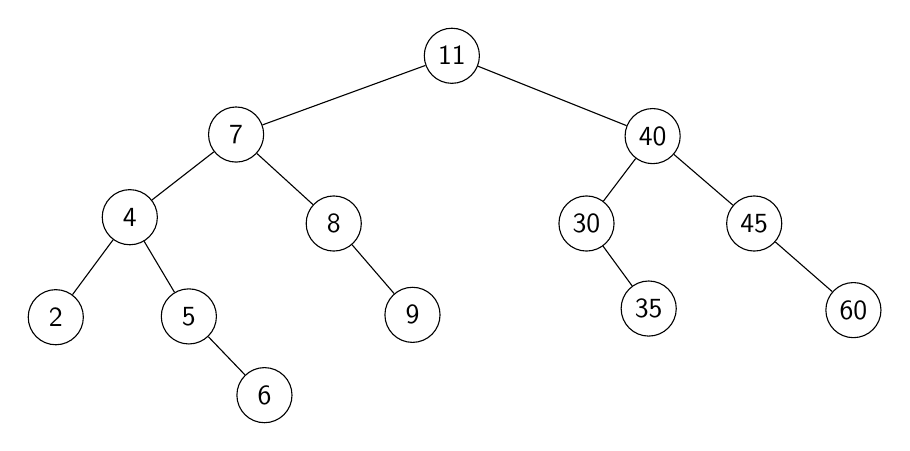
\begin{tikzpicture}[ every node/.style={font=\sffamily}, v/.style={circle,draw,minimum size=7mm,inner sep=0pt}]
\node[v] (11) at (5.03,0.00) {11};
\node[v] (7) at (2.29,-1.00) {7};
\node[v] (40) at (7.58,-1.02) {40};
\node[v] (4) at (0.94,-2.05) {4};
\node[v] (8) at (3.53,-2.13) {8};
\node[v] (30) at (6.74,-2.13) {30};
\node[v] (45) at (8.87,-2.13) {45};
\node[v] (2) at (0.00,-3.32) {2};
\node[v] (5) at (1.69,-3.31) {5};
\node[v] (9) at (4.53,-3.29) {9};
\node[v] (35) at (7.53,-3.21) {35};
\node[v] (60) at (10.13,-3.23) {60};
\node[v] (6) at (2.65,-4.31) {6};
\draw[] (11) -- (7);
\draw[] (11) -- (40);
\draw[] (7) -- (4);
\draw[] (7) -- (8);
\draw[] (4) -- (2);
\draw[] (4) -- (5);
\draw[] (5) -- (6);
\draw[] (8) -- (9);
\draw[] (40) -- (30);
\draw[] (40) -- (45);
\draw[] (30) -- (35);
\draw[] (45) -- (60);
\end{tikzpicture}%
\end{center}
\smallskip

Which of the following statements are correct?
\begin{enumerate}[label=(\Alph*)]
\item The deletion of 35 requires rebalance operations.
\item The insertion of 1 does not require rebalance operations.
\item After deleting 9, the nodes containing keys 4 and 7 become siblings in the new tree.
\item After successively deleting 35 and 60, the balance factor of the root in the new tree is 1.
\item After successively inserting 27, 28, and 29, the balance factor of the root in the new tree is -1.
\end{enumerate}
\end{pastexam}

\begin{pastsoln}
答案：(B)、(C)。

平衡因子 $\mathit{bf}(x) = $ 左子樹高度 $-$ 右子樹高度（資結書第~10.2~節），空樹高度算 $0$、葉子算 $1$。 原樹各節點的高度：
$6, 9, 35, 60, 2$ 是葉子（高度 $1$）；$5$、$8$、$30$、$45$ 高度 $2$；$4$ 高度 $3$（$\mathit{bf} = 1 - 2 = -1$）；$40$ 高度 $3$
（$\mathit{bf} = 0$）；$7$ 高度 $4$（$\mathit{bf} = 3 - 2 = 1$）；根 $11$ 高度 $5$（$\mathit{bf} = 4 - 3 = 1$）。 下面每個選項都從原樹
開始做。

\begin{itemize}
\item (A) 錯。 刪除葉子 $35$：$30$ 變成葉子，$\mathit{bf}(30) = 0$；$40$ 的左右子樹高度 $1$、$2$，$\mathit{bf} = -1$，高度仍是 $3$；
往上 $11$ 的右子樹高度沒變。 沒有節點的 $|\mathit{bf}|$ 超過 $1$，不必旋轉。
\item (B) 對。 插入 $1$：$11 \to 7 \to 4 \to 2$，成為 $2$ 的左子節點。 $\mathit{bf}(2) = 1$；$4$ 的左右高度變成 $2$、$2$，
$\mathit{bf}(4) = 0$，高度仍是 $3$，往上都不變。 不必旋轉。
\item (C) 對。 刪除 $9$：$8$ 變成葉子（高度 $1$）。 $7$ 的左子樹 $4$ 高度 $3$、右子樹高度 $1$，$\mathit{bf}(7) = 2$，失衡。
左子 $4$ 的 $\mathit{bf} = -1$，是 LR 型（資結書第~10.2.6~節）：先在 $4$ 左旋、再在 $7$ 右旋，$4$ 的右子節點 $5$ 轉上來。 結果
$5$ 的左子是 $4$（$4$ 的左子 $2$），右子是 $7$（$7$ 的子節點 $6$、$8$）。 $4$ 和 $7$ 成為兄弟。
\item (D) 錯。 刪除 $35$ 後如 (A)。 再刪除 $60$：$45$ 變成葉子，$40$ 的左右子樹都是高度 $1$，$40$ 的高度變成 $2$。 根 $11$ 的左子樹
高度 $4$、右子樹高度 $2$，$\mathit{bf} = 2$，失衡。 左子 $7$ 的 $\mathit{bf} = 3 - 2 = 1$，是 LL 型，在 $11$ 右旋：$7$ 成為根，
左子 $4$（高度 $3$），右子 $11$（$11$ 的左子 $8$、右子 $40$，高度 $3$）。 新根的 $\mathit{bf} = 3 - 3 = 0$，不是 $1$。
\item (E) 錯。 插入 $27$：$30$ 的左子節點，$\mathit{bf}(30) = 0$，高度仍是 $2$。 插入 $28$：$27$ 的右子節點；$27$ 高度 $2$，
$30$ 高度 $3$（$\mathit{bf} = 1$），$40$ 高度 $4$（$\mathit{bf} = 1$），根的左右高度都是 $4$，都沒有失衡。 插入 $29$：$28$ 的右子
節點，$\mathit{bf}(27) = -2$，右子 $28$ 的 $\mathit{bf} = -1$，是 RR 型，在 $27$ 左旋，$28$ 轉上來，左右是 $27$、$29$。 子樹高度回到
$2$，$30$、$40$、$11$ 的高度都和插入 $29$ 之前一樣：根的左子樹高度 $4$、右子樹高度 $4$，$\mathit{bf} = 0$，不是 $-1$。
\end{itemize}
\end{pastsoln}
